 \documentclass[%
 aps,
 prl,%
 amsmath,amssymb,
%preprint,%
 reprint,%
%author-year,%
%author-numerical,%
]{revtex4-1}

\usepackage{graphicx}% Include figure files
\usepackage{dcolumn}% Align table columns on decimal point
\usepackage{bm}% bold math
%My packages start
%\usepackage{subfig}
\usepackage{multirow}					
\usepackage{array}
%\usepackage{booktabs}
\usepackage{footnote} 
\newcommand{\angstrom}{\text{\normalfont\AA}}
\usepackage{booktabs}
\usepackage{float}
\usepackage{mathtools}
\usepackage{color}
\newcommand{\comment}[1]{\noindent \textcolor{blue}{#1}}
%My packages end
%\usepackage[mathlines]{lineno}% Enable numbering of text and display math
%\linenumbers\relax % Commence numbering lines

\begin{document}

\title[]{Accelerating atomic structure search with cluster regularization}% Force line breaks with \\

\author{K.\ H.\ S{\o}rensen}
\author{M.\ S.\ J{\o}rgensen}
\author{B.\ Hammer}
\email{hammer@phys.au.dk}
\affiliation{ 
Department of Physics and Astronomy, and Interdisciplinary Nanoscience Center (iNANO), Aarhus University, DK-8000 Aarhus C, Denmark.
}
% \homepage{phys.au.dk}
 
\date{\today}% It is always \today, today,
             %  but any date may be explicitly specified

\begin{abstract}
We present a method for accelerating the global structure optimization
of atomic compounds. The method is demonstrated to speed up the
finding of the anatase TiO$_2$(001)-(1$\times$4) surface
reconstruction within a tight-binding density functional theory (DFTB)
based evolutionary algorithm (EA) framework. As a key element of the
method, we use unsupervised machine learning techniques to categorize
the atoms in a diverse set of partially disordered surface structures
into clusters of atoms having similar local atomic
environments. Analysis of more than 1000 different structures show
that the total energy of the structures correlate with the summed
distances in feature space of the atomic environments to their
respective cluster centers, where the sum runs over all atoms in each
structure. Our method is formulated as a gradient based minimization
of this summed cluster distance for a given structure that alternates
with a standard gradient based energy minimization. While the latter
minimization ensures local relaxation within a given energy funnel,
the former enables escapes from meta-stable funnels and hence increases
the overall performance of the global optimization.
\end{abstract}

\pacs{Valid PACS appear here}% PACS, the Physics and Astronomy
                             % Classification Scheme.
\keywords{}%Use showkeys class option if keyword
                              %display desired
\maketitle

\section{\label{sec:introduction}Introduction}
In computational materials science, knowing the atomic structure of a
given molecule, atomic cluster or solid compound is a prerequisite for
further prediction of electronic and thermodynamic properties of such
a substance. In the emerging fields of combinatorial chemistry and
high-throughput computational screening of materials, the use of local
relaxation of probed structures is often sufficient since libraries of
molecular building blocks and crystal structures can be used to direct
the starting points for the searches. However, many problems exist for
which the structural motifs in the sought-after structures have no
analogues in known structures, and where global optimization must be
employed. A prominent example of this is that of surface relaxations,
that often exhibit structural motifs that are unique to a chemical
composition and crystaline polymorph as well as orientation. Dangling
Si-monomers and zig-zagging Si-dimers do for example evolve at the
Si(111)-(7$\times$7) and Si(001)-c(4$\times$2) surfaces, respectively, but
are otherwise not present in bulk Si or bulk-truncated Si surfaces. Likewise,
rutile and anatase TiO$_O$ single-crystal surfaces are known to exhibit
reconstructions and ad-structures, that have no equivalent in any TiO$_2$ bulk or surface systems.

Many strategies exist for performing global optimization in
conjunction with model potential or first-principles total energy
frameworks. Among these, stoichastic methods such as random search and
basin hopping are widely used and more advanced methods based on
evolutionary algorithms (EA) are becoming increasingly popular. Common
to these methods is the need for the perturbative update steps
followed by local relaxation and evaluation of whether or not to
retain the new structure. The nature of the perturbation steps ranges
from a mere rattling of the atomic positions to highly advanced
cross-over operations in which the atomic structure of several known
systems are combined. The exploration of configuration space is
ensured by the very stochastic nature of these updates, yet updates
that are too random will too often lead to rejection of the locally
relaxed structure and hence cause slow convergence. The atomic
displacement amplitude in a rattling update is a good example of
this. The amplitude must be kept small and sometimes only apply to a
subset of the atoms, as the new structural candidate otherwise become
too unstable.

The present work aims at formulating a means of performing a random
update in a way that optimizes the chances of finding more stable
structural candidates in subsequent local relaxation steps. The method
proposed starts from assigning every atom in a given structure to a
cluster of similar atoms present in a reference set of structures.
The similarity is measured as the distance in a feature space, chosen
sufficiently simple that it can be illustrated. With every atom
assigned to a cluster, we evaluate for a given structure the sum of
the distances in feature space of the atoms from their respective
cluster centers. This structure specific scalar measure of distance to
cluster centers is demonstrated to correlate with the structure
stability -- the lower the distance measure, the more stable the
structure. As a consequence, minimizing the cluster distance measure
contains an element of bringing a structure into a region of
configuration space that is expectedly more stable. The minimization
can be done by moving opposite to an analytic gradient and has
potential to take a structure out of local energy minima, since the
cluster distances are measured in a space that is complementary to the
energy landscape. We refer to our method as the
\textit{cluster regularization method} as it penalizes large cluster
distances.

The paper is outlined as follows: In the Methods section we present
the computational setup and outline the reference method used. In
Theory section we describe the components of our method, including the
choice of feature vector and the clustering technique. In the Results
section, the method is used in full scale global optimization in
search for the anatase TiO$_2$(001)-(1$\times$4) surface
reconstruction. This section demonstrates the usefulness of the method
and further investigates its efficacy as the number of unknown atomic
position is increased in the global optimization.





\begin{figure}[h]
    \centering
    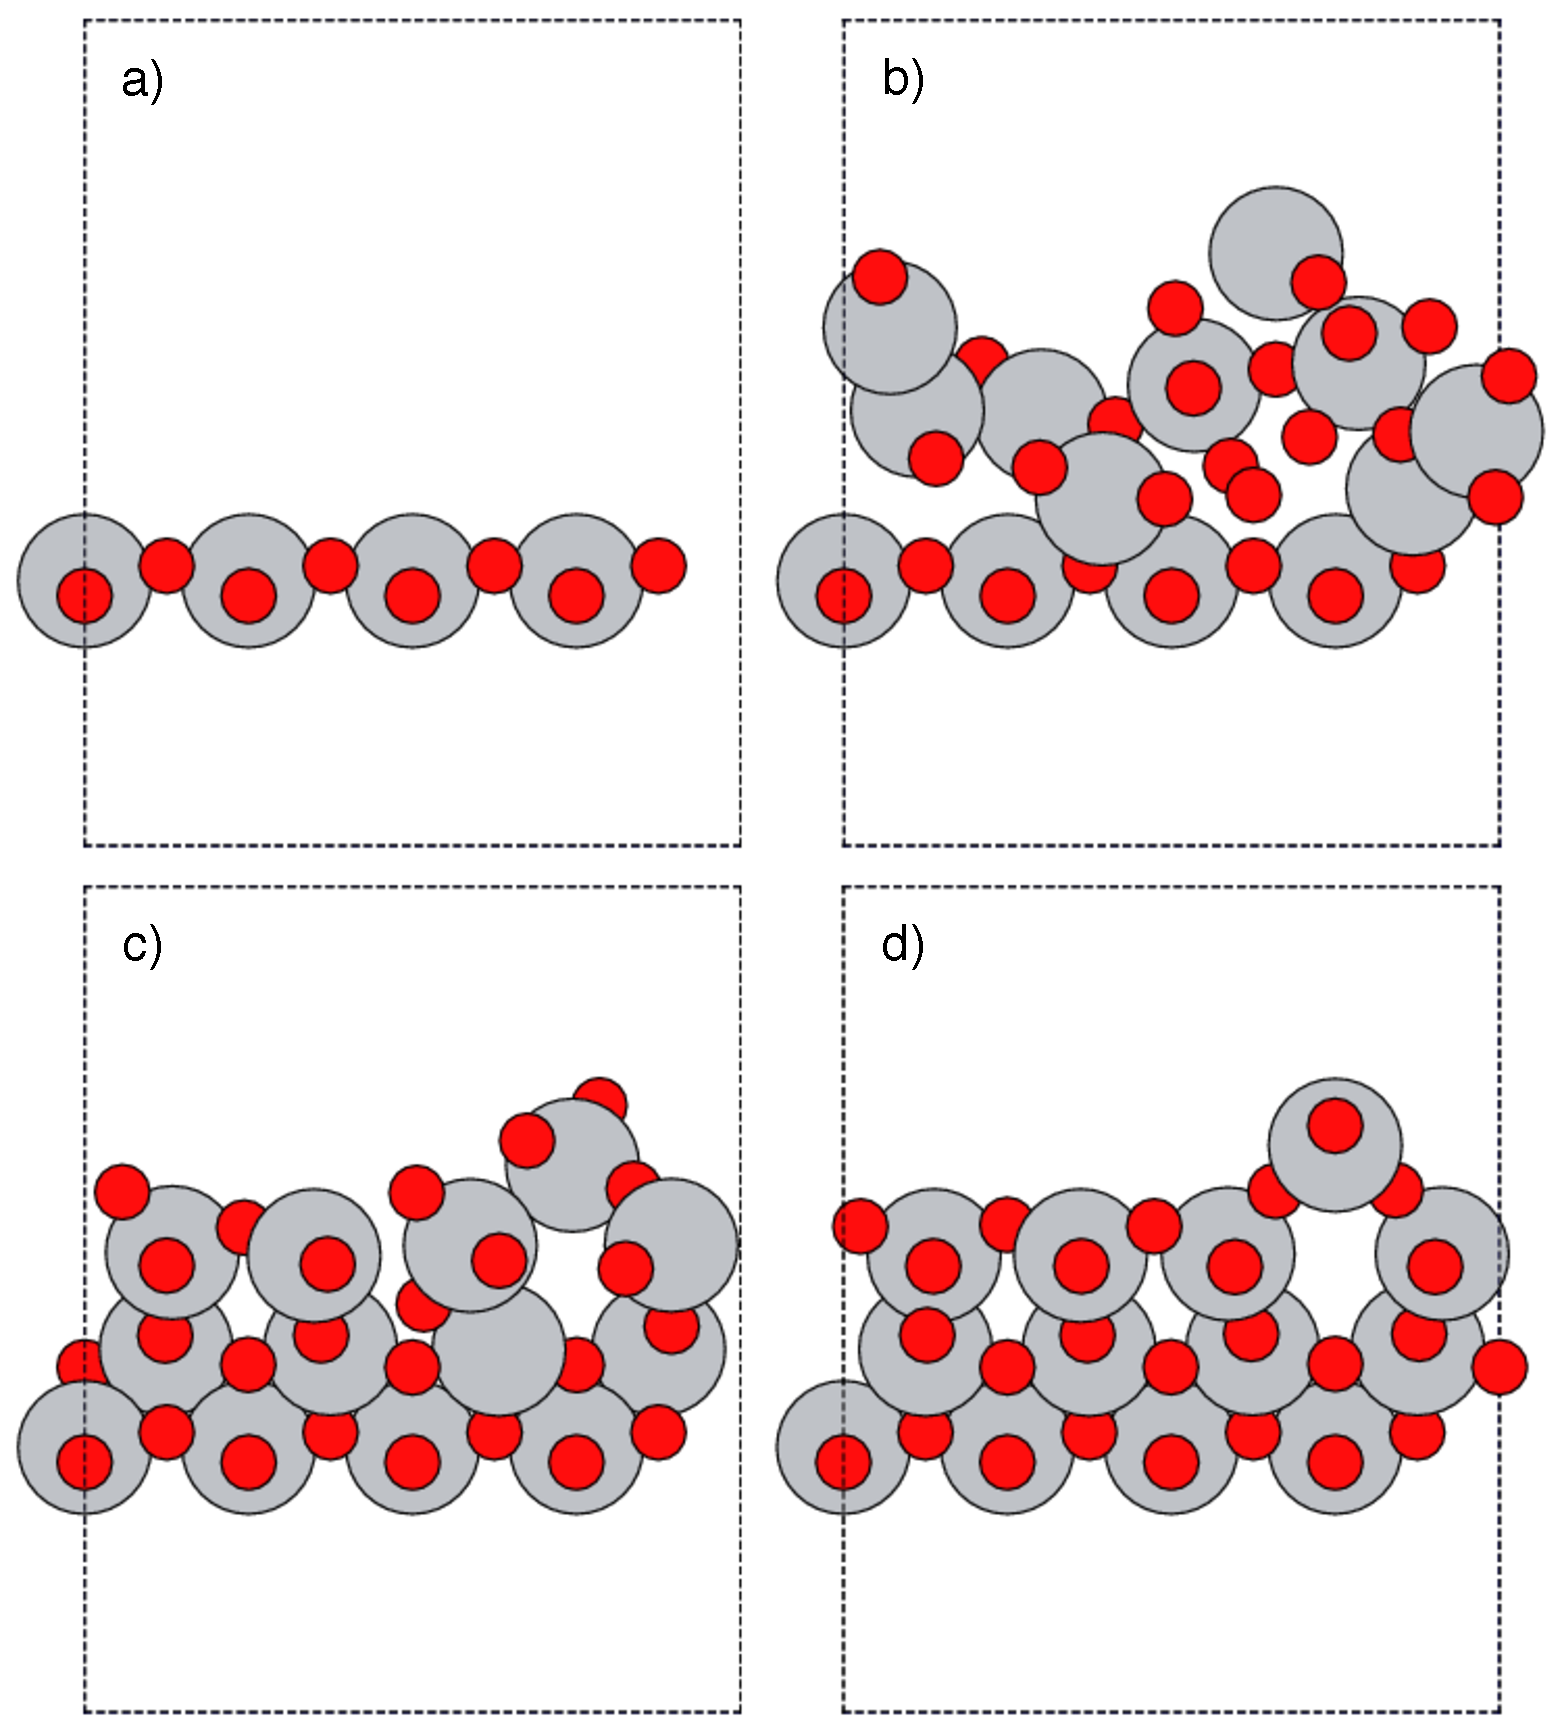
\includegraphics[width=1.0\columnwidth]{fig1-intro.pdf}
    \caption{Example of the Ti$_{n}$O$_{2n}$ structures we are working with. Top-left the slab used, top-right a initial structure, bottom-left a structures with some minimisation, bottom-right the global mimimum.}
    \label{figintro}
\end{figure}



\section{The method}
What we are contributing in this article is a method we call cluster regularization. 
It is a way to impose symmetry into the search without specifying the symmetry explicit, 
as pointed out in \cite{Pikard2011} low energy structures tend to have a very high degree of symmetry.

The method first constructing a feature vector for each atom, then cluster this feature vectors, and at last update the atomic positions such that the distance between the feature vectors and the cluster centers are minimized.   

\subsection{Atomic features}
 
The atomic features vectors used in this study is inspired from Botu and Ramprasad \cite{Botu2015} and also used by Xin Chen \cite{Chen2017}.

The length of our feature vector is the number of atomic types plus one. For our system with 2 atomic types the atomic feature vector have length 3.

The first 2 components for each atom $i$, is calculated by finding the list of neighbors $nl(i)$ within a cutoff radius $c$. For each of the 2 atomic types T we calculate. 

\begin{equation}
f_T(i) = \sum_{\mathclap{j \in nl(i,c);T=T(j)}} e^{-d_{ij}/1\text{\AA}}f_c(d_{ij})  \label{eq1}
\end{equation}

Here T(j) is the atomic number of the j'th atom. $d_{ij}$ is the distance $|\vec r_{ij}|=|\vec r_j- \vec r_i|$ from the i'th to the j'th atom in {\AA}ngstr\"{o}m. The last component of the atomic feature vector is $T(i)$ the atomic number for atom i. 
The function $f_c$ make sure that an atoms contribution vanish at the cut-off radius, this gives the gradient higher stability.

\begin{equation}
f_c(d)={{\cos(\pi*d/c)+1}\over 2}
\end{equation}


In figure \ref{fig_feature} the feature vector is displayed for 1019 structures of Ti$_{13}$O$_{26}$ with the first component $f_8(i)$ along the x-axis, the second $f_{22}(i)$ along the y-axis and the color is given by the third component $T(i)$. 


\begin{figure}[h]
    \centering
    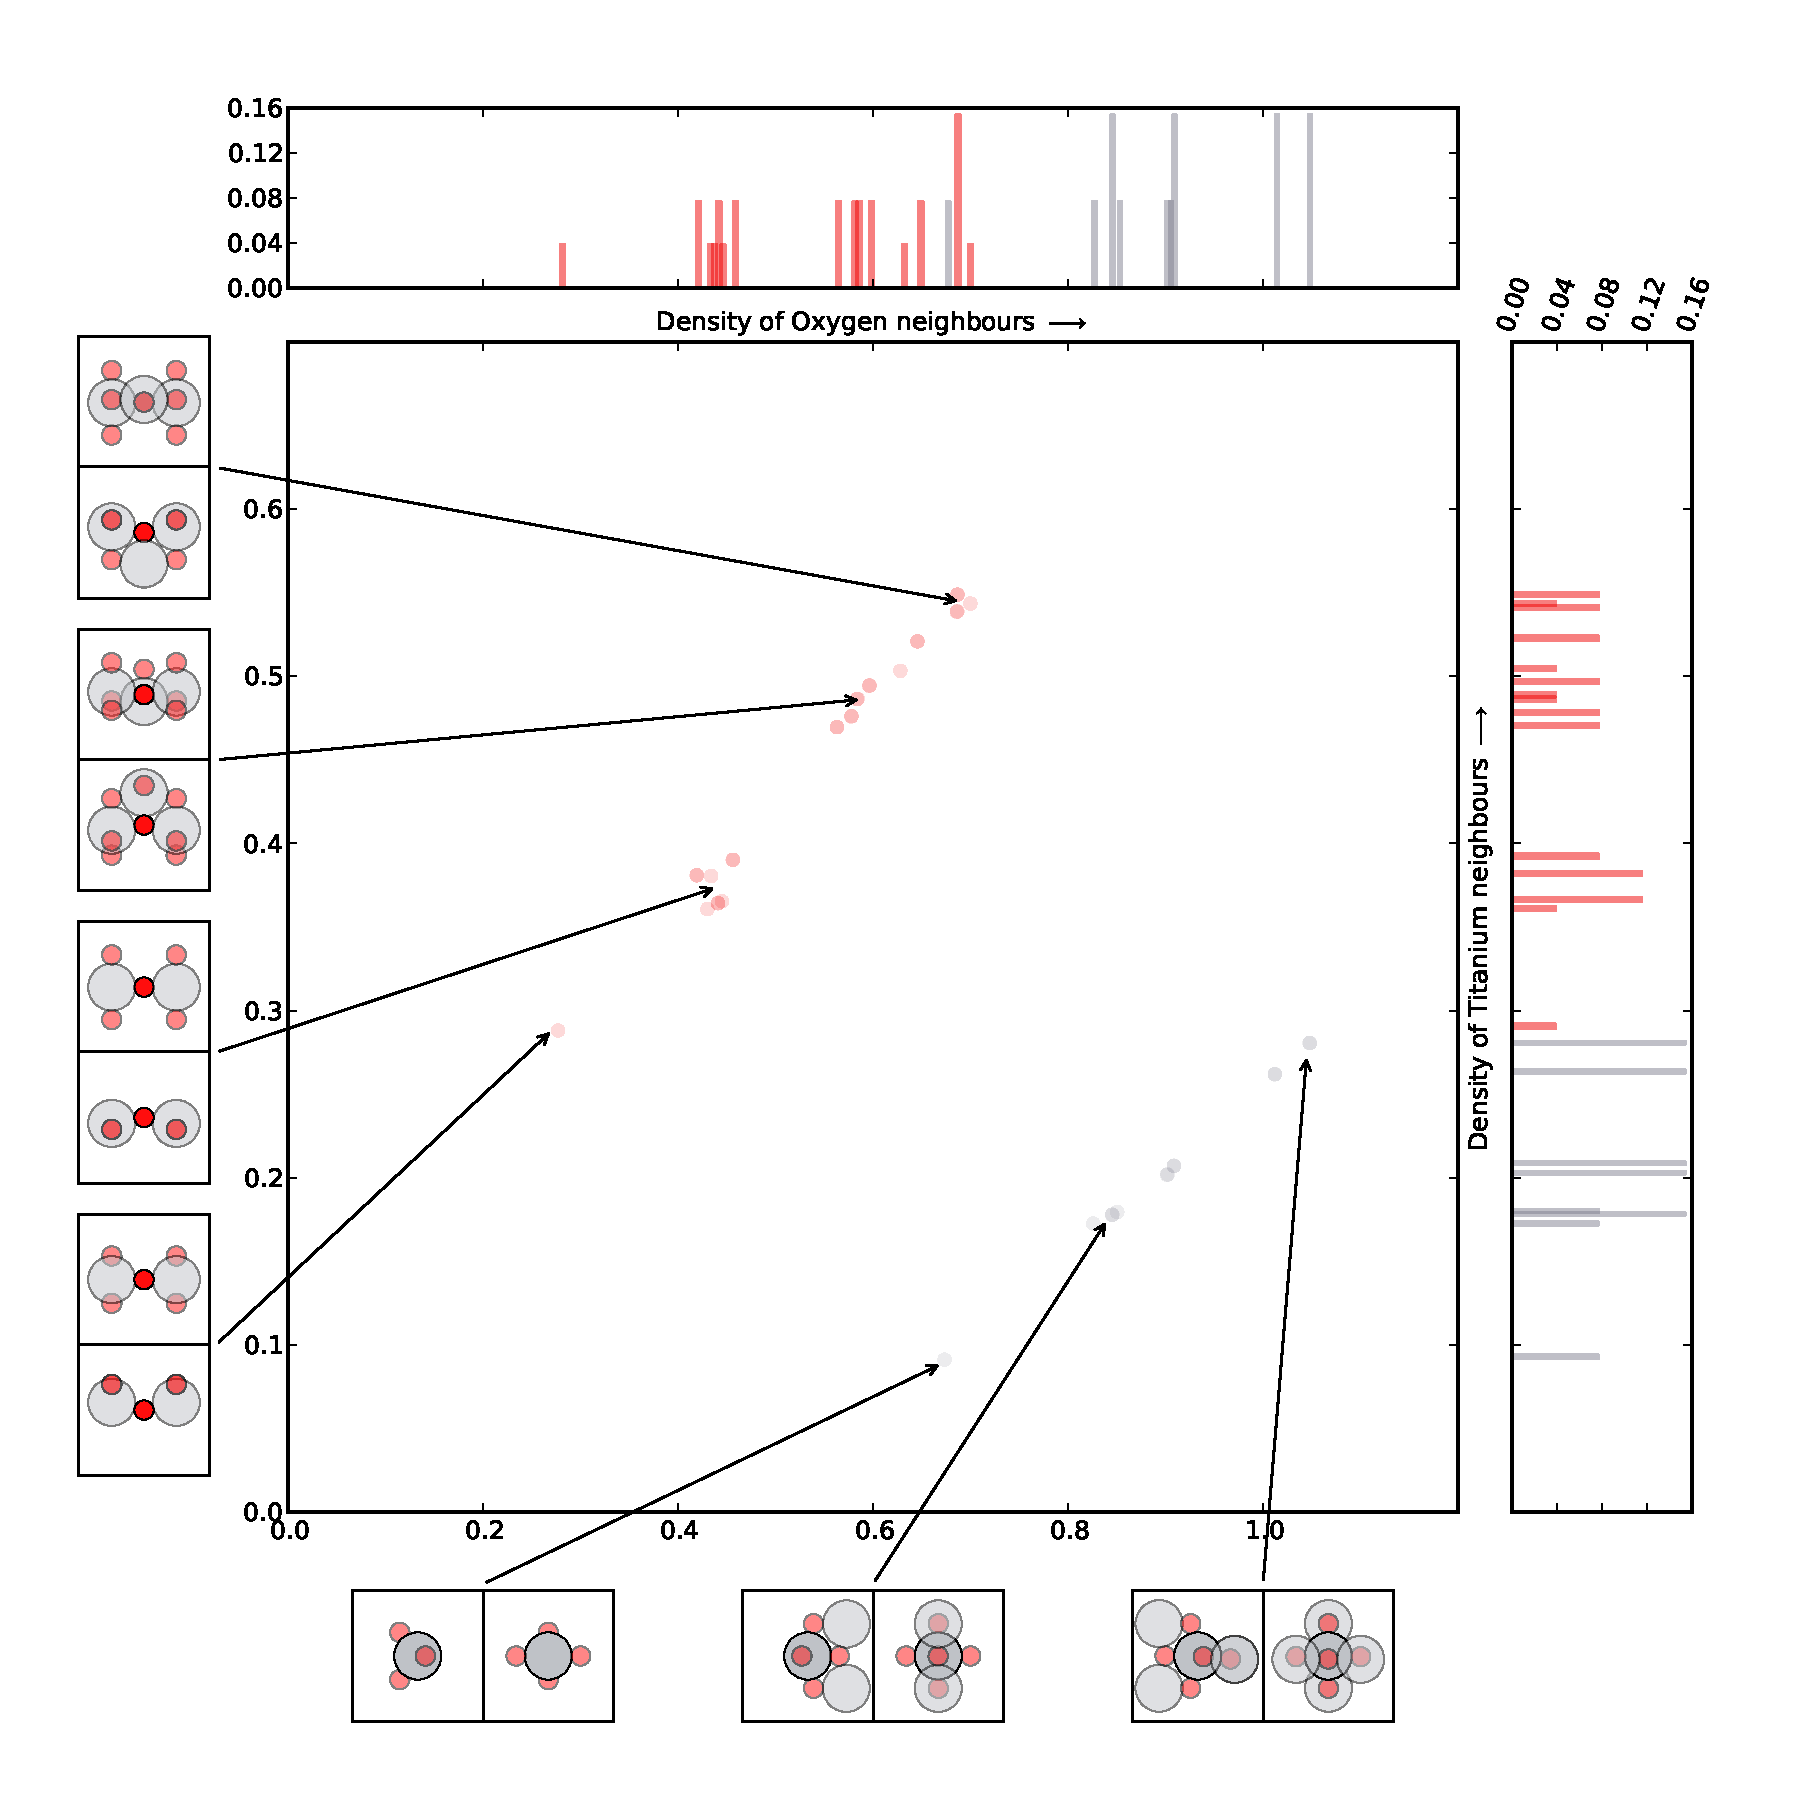
\includegraphics[width=1.0\columnwidth]{fig2-gm_scatterplot.pdf}
    \caption{Visualization of global minimum for Ti$_{13}$O$_{26}$ structures in feature space}   
    \label{fig_global}
\end{figure}



\begin{figure}[h]
    \centering
    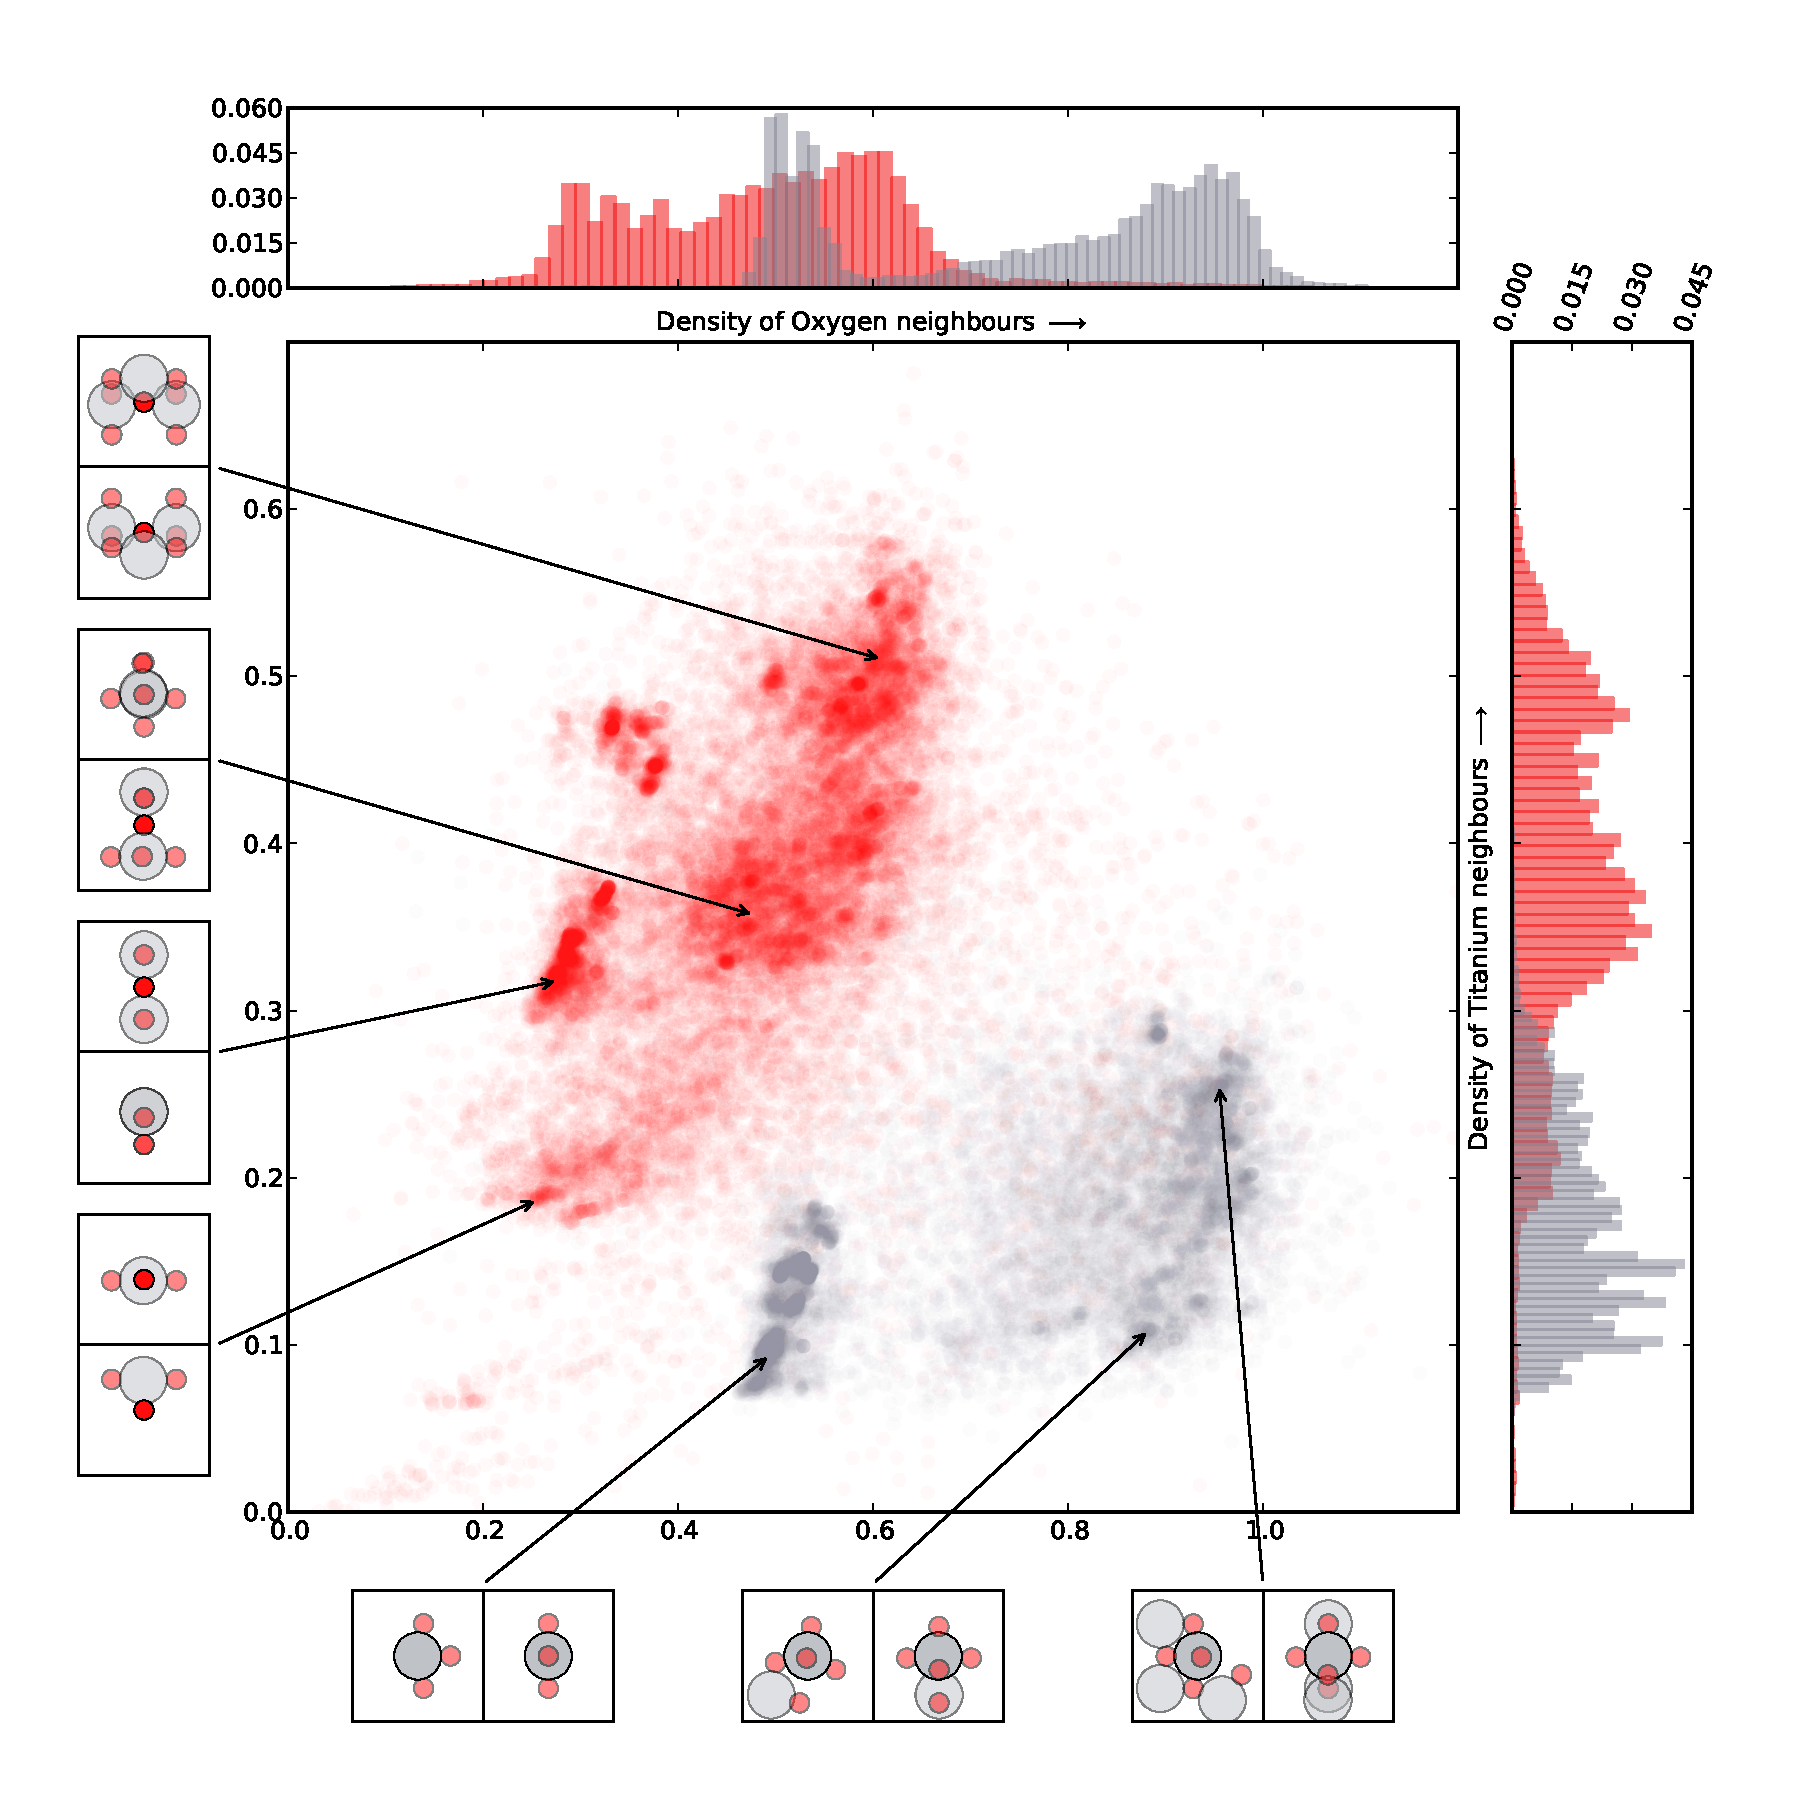
\includegraphics[width=1.0\columnwidth]{fig3-scatterplot.pdf}
    \caption{Visualization of atoms from 1019 Ti$_{13}$O$_{26}$ structures in feature space}   
    \label{fig_feature}
\end{figure}




\subsection{Clustering}
The clustering method used is this study is k-means with 2
modifications. The first is a modification to avoid generating empty
clusters \cite{Malay2009} and the second modification is using
k-means++ cluster initialization. While working with clustering on the
atomic feature vectors, the total cluster distance vs. energy correlation
illustrated on figure \ref{fig_corr} was discovered. 

\begin{figure}[h]
    \centering
    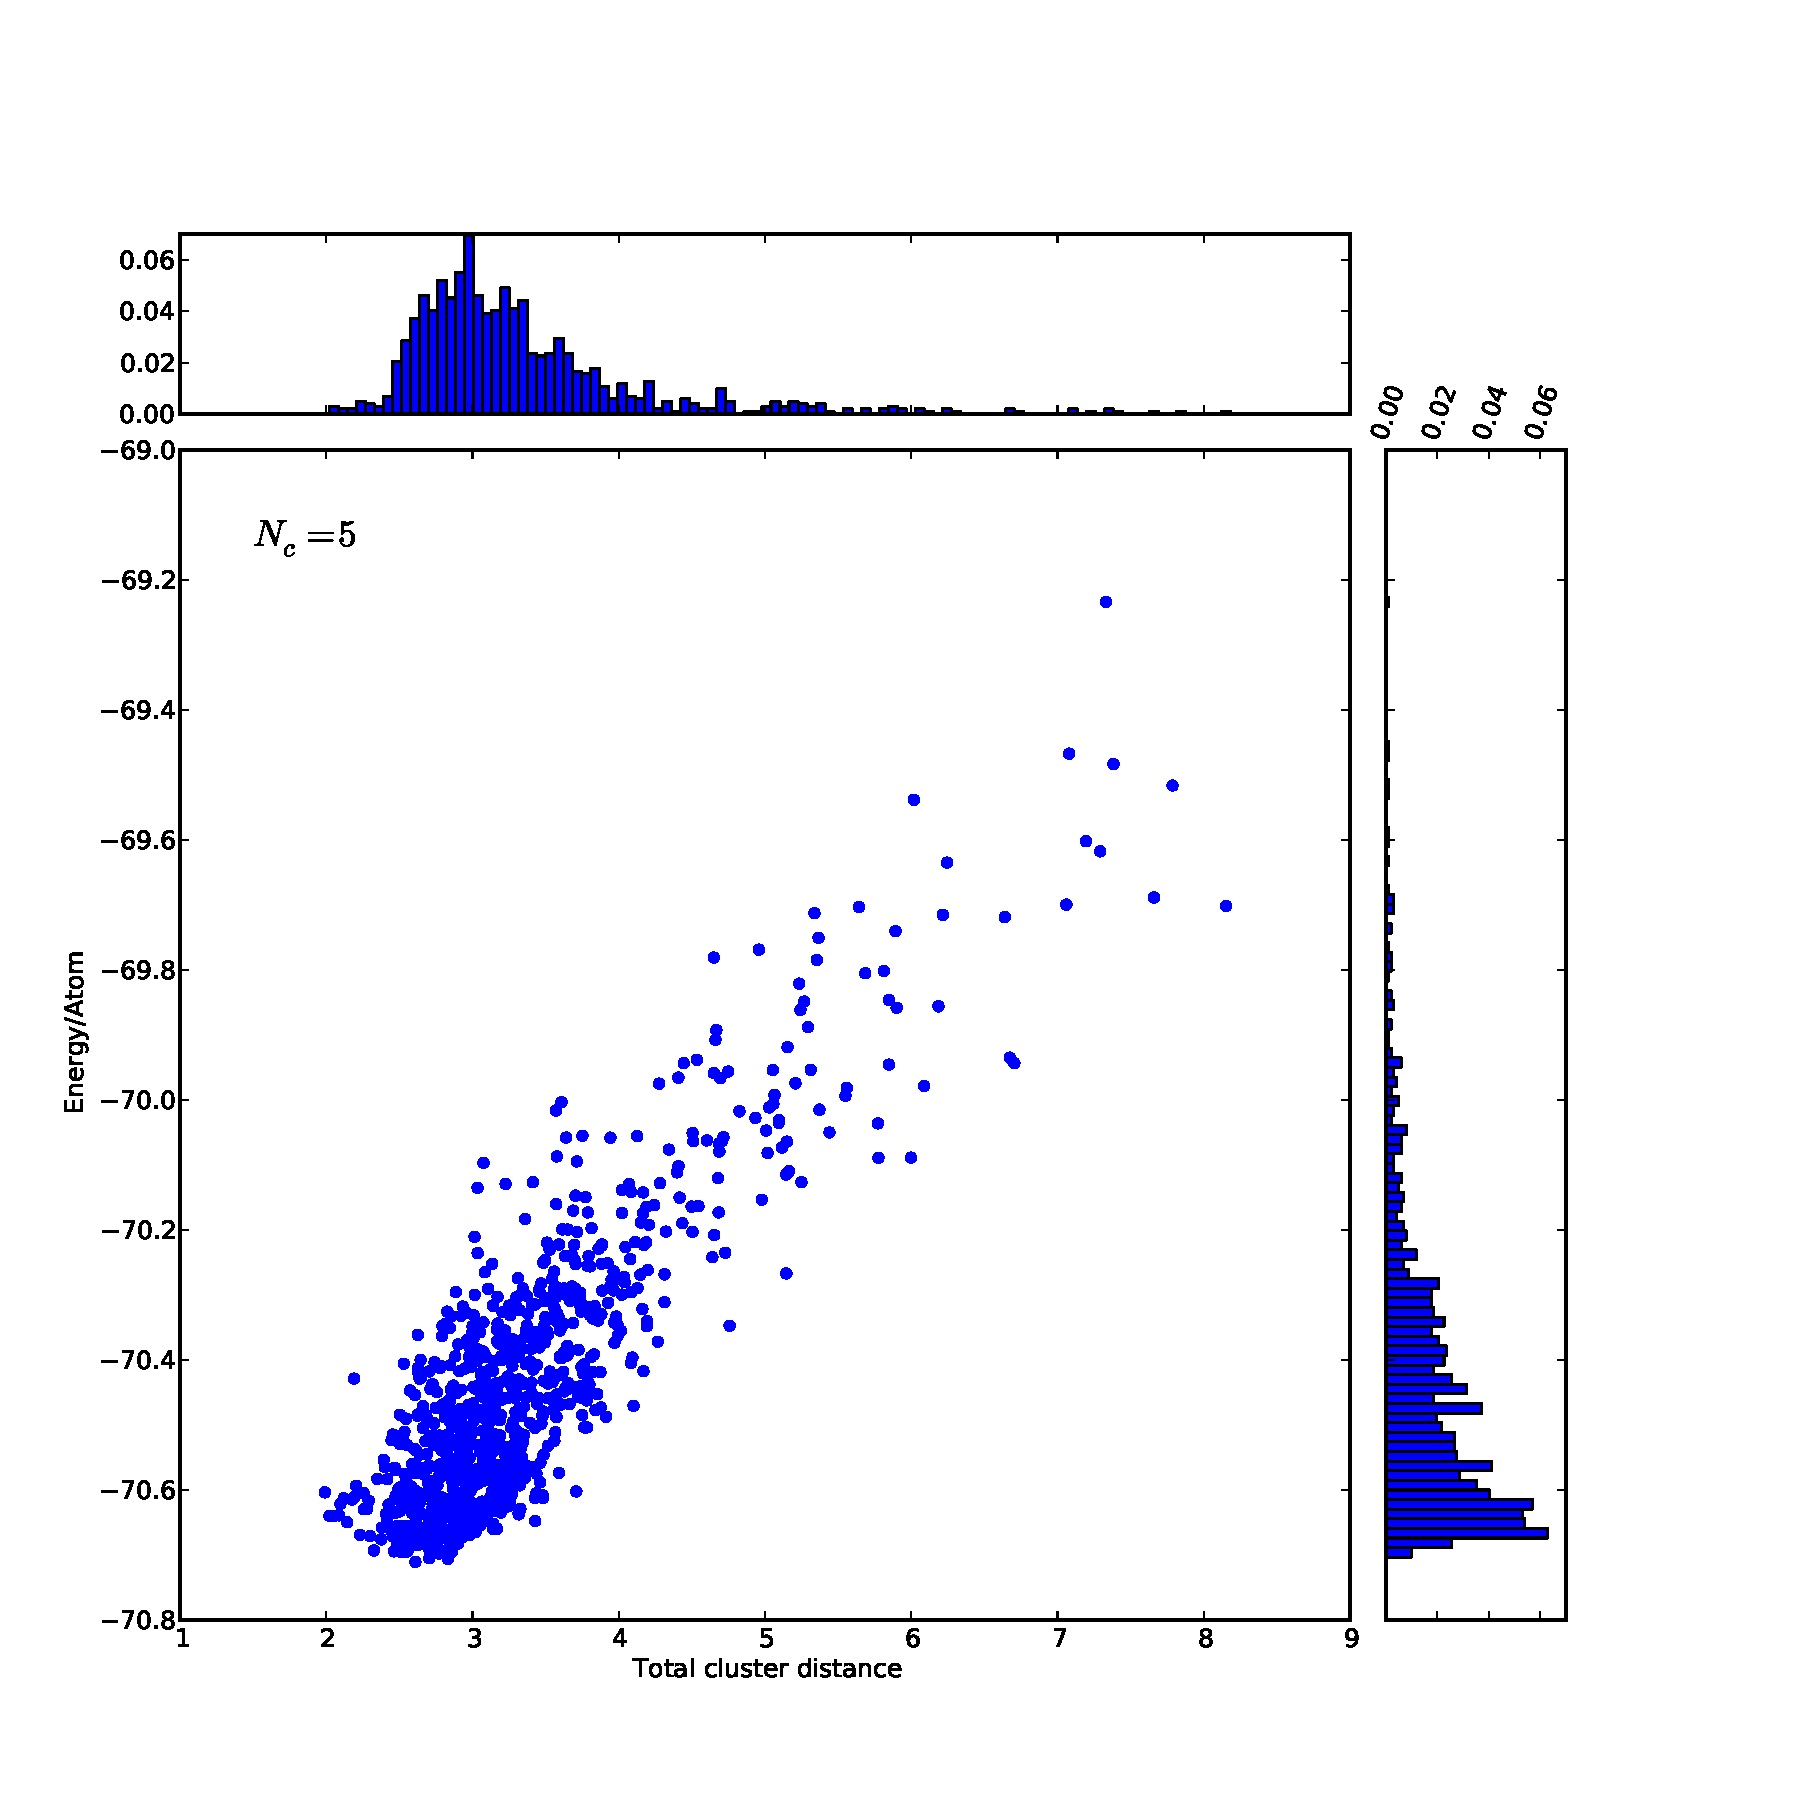
\includegraphics[width=1.0\columnwidth]{fig4-correlation.pdf}
    \caption{Cluster distance vs. energy correlation}
    \label{fig_corr}
\end{figure}

It was immediately recognized that it could be applied to speed up the search for minimum energy structures.
It is our suspicion that the better the correlation the higher the speedup, 
but we haven't done a formal study of this. We have observed that regular structures like bunk and surface have better correlation than molecules. Another factor influencing the correlation is the choice of feature vector, 
unlike other machine learning methods this type of clustering don't ignore noisy features, so the features should be chosen with care.  
 
Given an atomic structure $S$ (a list of atoms) the total cluster distance is given by:
\begin{equation}
\text{TCD}(S) = \sum_{i \in S} d(\vec f(i), \vec c_i) \label{eq3}
\end{equation}
For each atom $i$ in $S$ we calculate the feature vector $\vec f(i)$ then 
assign it to a cluster center $\vec c_i$.   
The sum over the distance between $\vec f(i)$ and $\vec c_i$ for all atoms $i$ in a structure $S$ 
gives the total cluster distance $TCD(S)$.
In the case of figure \ref{fig_corr} the cluster centers is found by clustering over all atomic feature vectors 
for the 1019 structures in the data set. 

\subsection{Cluster regularization}
Because the all but the last components of our feature vector is analytical functions of the atomic coordinates, one can derive the analytical gradient. 
Now we can minimize the cluster distance by following the negative gradient to a local minima. 

Then we switch and minimize the energy with DFTB+ and then minimize cluster distance again. Figure \ref{fig_min} shows the process. The idea is that alternate the two minimizations they will help each other out of there local minima and further down in energy and cluster distance.
   
\begin{figure}[h]
    \centering
    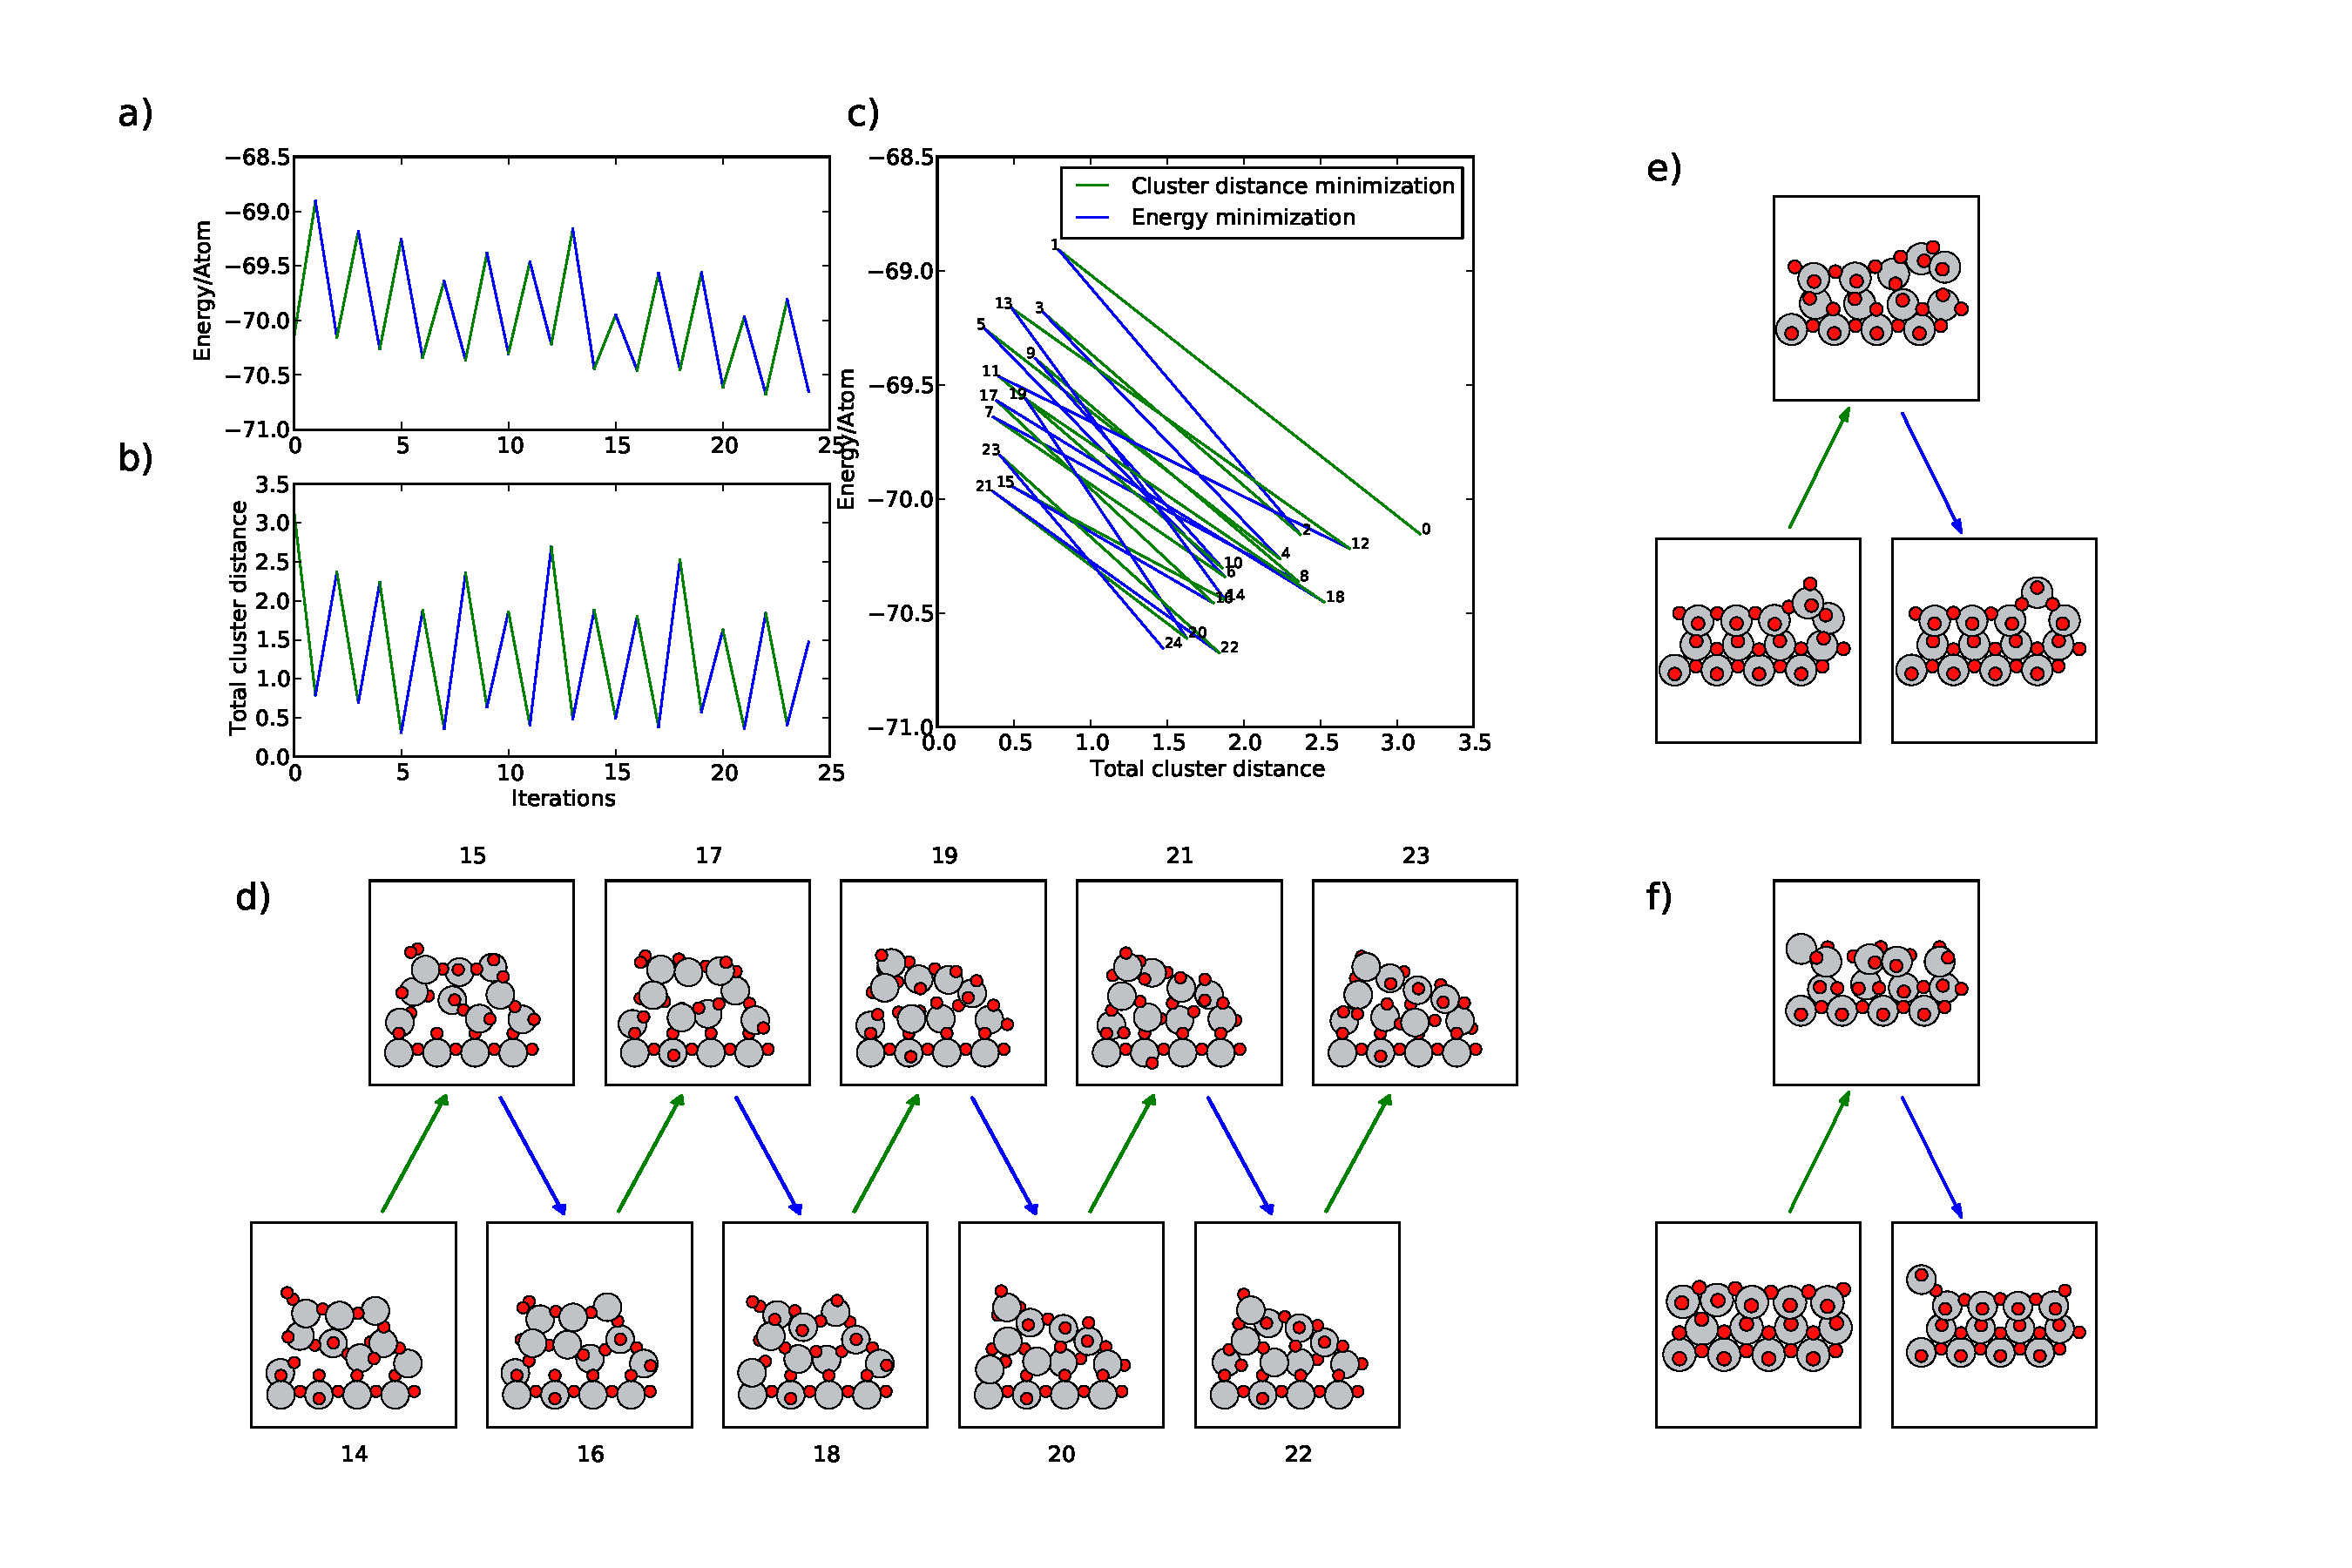
\includegraphics[width=1.0\columnwidth]{fig5-minimize.pdf}
    \caption{Green lines and arrows shows a cluster distance (cd) minimization and the blue DFTB+ relaxations. Here the first/bottom layer is the template. While it is hard to see progress in individual minimization step there is small details to notice on the plot. Notice that in the cd. step from 16 to 17 the hole in the second layer is filled and that in the cd. step from 18 to 19 the 2 oxygen atoms in top left corner is split up.}
    \label{fig_min}
\end{figure}


\section{Testing}

\subsection{Test setup}
To test the technique we implemented cluster regularization as a mutation operator in ASE's genetic algorithm (ga)\cite{ase_ga} framework. 
The mutation operator takes a list of parents and the execute the following steps:
\begin{enumerate}
\item Calculate atomic features for all parents.
\item Cluster them and find cluster centers.
\item Copy the lowest energy parent to the child
\item minimize cluster distance of child.
\item return child.
\end{enumerate}
When the mutation returns the child then the ga will make a energy relaxation 
and we have a cycle as illustrated in figure \ref{fig_min}.

To establish a benchmark the ga with bayesian hyper-parameter optimization (BHO.) search was run on the 3 layer system.
Run with cut\&splice, permutation and rattle mutations the search found the optimal ratios was 59\% cut\&splice, 0\% permutation, 41\% rattle. 

Next we did a BHO. search for the best parameters for cluster regularization, we found that 5 clusters, 3 parents and cutoff radius c=11.9 gave the best results.

Last we did a BHO. search for the best combination of cluster regularization, cut\&splice and rattle, we found that 70\% cluster regularization, 28\% cut\&splice and 2\% rattle did well.

We tested these 3 methods on a 2 layer, 3 layer and a 4 layers system. 

\subsection{Test result}

On figure \ref{fig_success} we see that pure cluster reg. (orange curve) start finding minimum structure much faster than the benchmark (yellow curve) , but it levels out around 60-70\%. The problem is that cluster regularization and energy minimization have local minima close to each other and running the algorithm make them switch between this minima. When cluster regularization is mix with other mutations (red curve) the problem disappear. 

\begin{figure}[h]
    \centering
    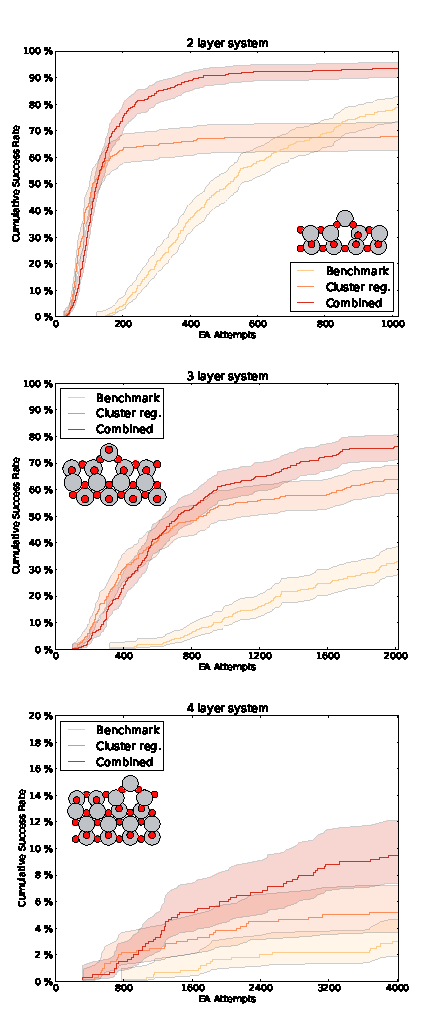
\includegraphics[width=1.0\columnwidth]{fig6-success.pdf}
    \caption{Cumulative success for 2,3 and 4 layer systems}
    \label{fig_success}
\end{figure}

With the 3 layers system on figure \ref{fig_success} the problem isn't as prominent which might be because there is more free variables in this problems. Else we observe the same as the 2 layer system combined and pure cluster reg. does better than the benchmark. Pure cluster reg. does better in the start but is overtaken by the combined method later on. 
In the 4 layer system the tendency continues but the success rate is much lower and we made double as many runs to shrink the confidence intervals. 

\section{Analysis}
In \cite{Pikard2011} it is shown that the number of local stable configuration in a system is 
\begin{equation}
n_s(N) = e^{\alpha N}
\end{equation}


If we take the number of found minimas and divide with the number of attemts used. 
We get the probability of finding the global minima.

\begin{equation}
p_{gm} ={ \text{Number of found minimas}\over \text{Number of attemts}}
\end{equation}

If we generated random structure and relaxed them it would be reasonable to assume that 

\begin{equation}
p_{gm} \propto   {1 \over e^{\alpha N}}
\end{equation}



In figure \ref{fig_scale} $p_{gm}$ is plotted for our 3 methods.


\begin{figure}[h]
    \centering
    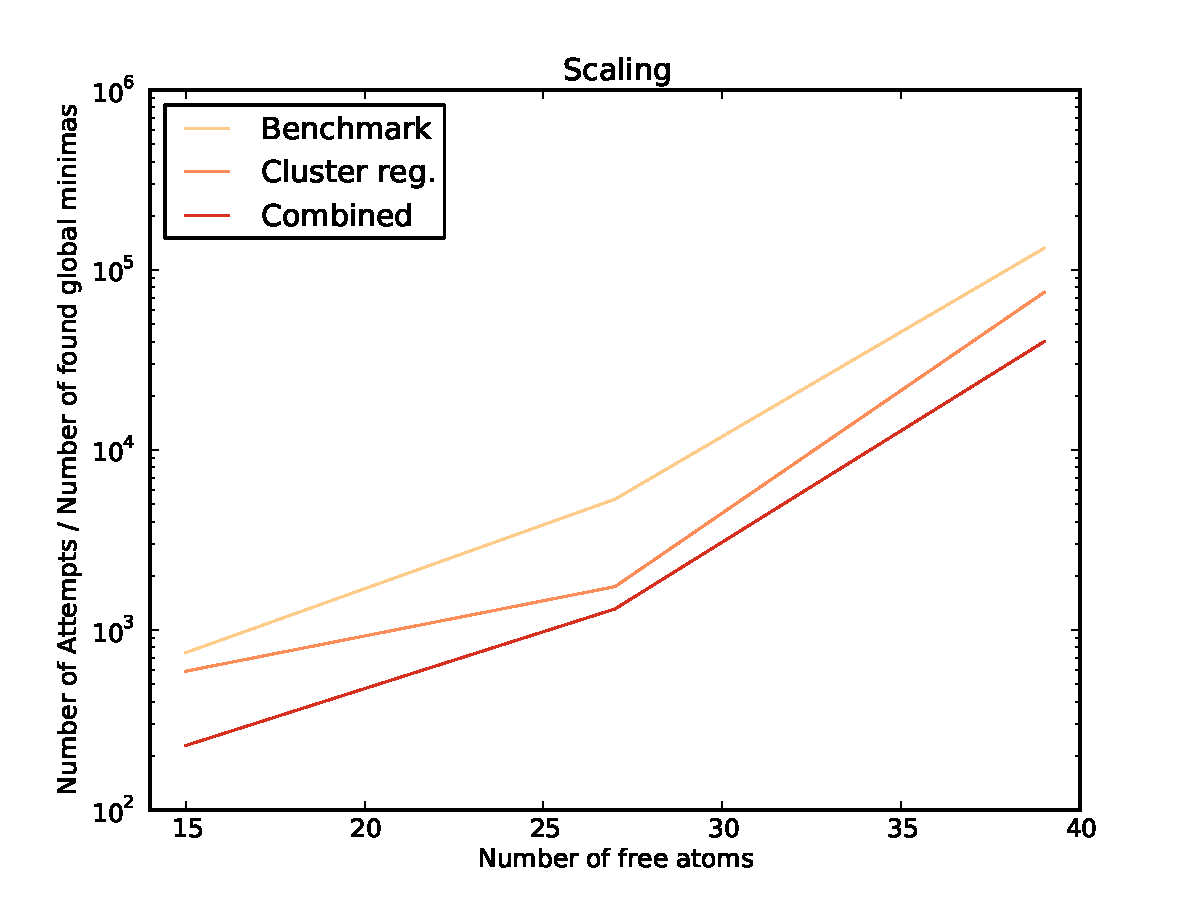
\includegraphics[width=1.0\columnwidth]{fig7-scaling.pdf}
    \caption{}
    \label{fig_scale}
\end{figure}


We observe that the lines is almost linear with a little kink at the middle. The kink is properly due to overfitting because the 3 layer system was use to fit the hyperparameters.  

We can fit the line on the semilog plot too the form.

\begin{equation}
p_{gm} = e^{a N + b}
\end{equation}

Now we want to define some good metrics to measure the performance of our search algorithms.
We define the search speed as $s_\text{search}= e^b$ and the scaling factor $f_\text{scale}=-1.0/a$,
both is define such that higher values would require lesser attemts.

Now the relation about can be written as. 

\begin{equation}
p_{gm} = s_{\text{search }} e^{N / f_\text{scale}}
\end{equation}


From our fit we get the following results from our 3 methods.


\begin{center}
  \begin{tabular}{ | l | c | c | }
    \hline
    Method & $s_{\text{search}}$ & $f_\text{scale}$ \\  
    \hline
    Benchmark & 0.042 & 4.638 \\ 
    Cluster reg. & 0.055 & 4.952 \\ 
    Combined  & 0.146 & 4.644 \\
    \hline
  \end{tabular}
\end{center}


We notice that the search speed of the resulting method is 3.5 times greater than the search speed of the benchmark method.












\section{Conclusion}

We acknowledge support from the Danish Council for Independent Research | Natural Science (grant no. 0602-02566B) and from VILLUM FONDEN (Investigator grant, project no. 16562).

\begin{thebibliography}{12}  
\bibitem{Starke1998} U. Starke \textit{et al}., Phys. Rev. Lett. \textbf{80}, 758 (1998).    
\bibitem{Malay2009} {A Modified k-means Algorithm to Avoid Empty Clusters} Malay K. Pakhira, International Journal of Recent Trends in Engineering, Vol 1, No 1, May 2009
\bibitem{Pikard2011}  {Ab initio random structure searching} Chris J. Pickard and R. J. Needs. J. Phys.: Condens. Matter \textbf{23} (2011) 053201 (23pp) DOI:10.1088/0953-8984/23/5/053201
\bibitem{Botu2015} {Adaptive Machine Learning Framework to Accelerate Ab Initio Molecular Dynamics.} V. Botu and R. Ramprasad, Int. J. Quantum Chem. 2015, 115 ,1075-18083. DOI:10.1002/qua.24836    
\bibitem{Chen2017} {Understanding atomic chemistry with machine learning.} Chen, X., J�rgenson, M. S., Hammer, B., \& Li, J. (2017) Unpublished
\end{thebibliography}


\end{document}
